\documentclass[twoside]{report}
\usepackage[utf8]{inputenc}
%\usepackage[english]{babel}
\usepackage{amsthm}
\usepackage{tkz-fct} 
\usepackage{thmtools}
\usepackage[margin=1in]{geometry}
\usepackage{amsmath,amssymb}
\usepackage{multicol}
\usepackage{graphicx}
\usepackage{tikz}
\usepackage{listings}
\usetikzlibrary{positioning} 
\usetikzlibrary{calc,patterns,angles,quotes}
\usetikzlibrary{calc,arrows, arrows.meta}
\tikzset{
  arrow/.pic={\path[tips,every arrow/.try,->,>=#1] (0,0) -- +(.1pt,0);},
  pics/arrow/.default={triangle 90}
}
\usepackage{pgfplots}% also loads graphicx
\pgfplotsset{compat=1.11} %width=10cm,
\usetikzlibrary{backgrounds}
\usepackage{siunitx}
\sisetup{per-mode=fraction} %,fraction-function = \nicefrac}
\DeclareSIUnit{\gallon}{gal}
\usepackage{fancyhdr}
\usepackage{pst-node}
\psset{nodesep=2pt,linearc=2pt,arrows=->,linecolor=blue,arrowinset=0}
\def\lbl#1{\ncput*{\text{\tiny #1}}}
\usepackage{xcolor}
\usepackage{tcolorbox}
\usepackage{lmodern}
\usepackage{relsize}
\newcommand{\highlight}[1]{%
  \colorbox{red!50}{$\displaystyle#1$}}
\usepackage{url}
\usepackage{cancel}
\usepackage{float}
\usepackage[numbers]{natbib}
\usepackage{setspace}
\usepackage{subcaption}
\usepackage{varwidth}
% set the arrows as stealth fighters (personal preference)
\tikzset{>=stealth}
\captionsetup[figure]{labelfont={bf},name={Figure},labelsep=period}

\declaretheoremstyle[
  spaceabove=6pt, spacebelow=6pt,
  headfont={\color{blue}\fontfamily{cmss}\selectfont\bfseries},
  notefont=\fontfamily{cmss}\selectfont\bfseries, notebraces={(}{)},
bodyfont=\fontfamily{cmss}\selectfont\itshape,
  postheadspace=1em,
]{mystyle}
\declaretheorem[style=mystyle,numbered=no]{definition}
\declaretheorem[style=mystyle,numbered=no]{lemma}

\declaretheoremstyle[
  spaceabove=6pt, spacebelow=6pt,
  headfont={\color{black} \fontfamily{cmss}\selectfont\bfseries},
  notefont=\fontfamily{cmss}\selectfont\bfseries, notebraces={(}{)},
bodyfont=\fontfamily{cmss}\selectfont,
  postheadspace=1em,
  qed=$\triangle$
]{mystyle2}
\declaretheorem[style=mystyle2,numbered=no]{remark}

\declaretheoremstyle[
  spaceabove=6pt, spacebelow=6pt,
  headfont={\color{orange} \fontfamily{cmss}\selectfont\bfseries},
  notefont=\fontfamily{cmss}\selectfont\bfseries, notebraces={(}{)},
bodyfont=\fontfamily{cmss}\selectfont,
  postheadspace=1em,
  qed=$\triangle$
]{mystyle3}
\declaretheorem[style=mystyle3,numbered=no]{example}

\declaretheoremstyle[
  spaceabove=6pt, spacebelow=6pt,
  headfont={\color{blue} \fontfamily{cmss}\selectfont\bfseries},
  notefont=\fontfamily{cmss}\selectfont\bfseries, notebraces={(}{)},
  bodyfont=\fontfamily{cmss}\selectfont\itshape,
  postheadspace=1em,
  qed=
]{mystyle4}
\declaretheorem[style=mystyle4,numbered=no]{law}

\declaretheoremstyle[
  spaceabove=6pt, spacebelow=6pt,
  headfont={\color{blue} \fontfamily{cmss}\selectfont\bfseries},
  notefont=\fontfamily{cmss}\selectfont\bfseries, notebraces={(}{)},
bodyfont=\fontfamily{cmss}\selectfont,
  postheadspace=1em,
  qed=
]{mystyle5}
\declaretheorem[style=mystyle5,numbered=no]{strategy}

\declaretheoremstyle[
  spaceabove=6pt, spacebelow=6pt,
  headfont={\color{blue} \fontfamily{cmss}\selectfont\bfseries},
  notefont=\fontfamily{cmss}\selectfont\bfseries, notebraces={(}{)},
bodyfont=\fontfamily{cmss}\selectfont\itshape,
  postheadspace=1em,
  qed=
]{mystyle6}
\declaretheorem[style=mystyle6,numbered=no]{theorem}


\renewcommand{\qedsymbol}{\rule{0.7em}{0.7em}}
\renewenvironment{proof}{{\bfseries \fontfamily{cmss} \scshape Proof:}}



\newcommand{\reporttitle}{###}
\newcommand{\reportauthor}{Kai Cooper}
\newcommand{\reportsecondauthor}{}
\newcommand{\reportthirdauthor}{}
\newcommand{\reportfourthauthor}{}
\newcommand{\reportfifthauthor}{}
\newcommand{\supervisor}{Dr. Medhi Ghoulam}

\date{June 2021}

\renewcommand{\chaptername}{Part}
\newcommand{\lap}{\nabla^2}
\newcommand{\dif}[1]{\text{d}#1}

\newcommand{\code}{\texttt}

\definecolor{fcolor}{RGB}{0,255,255}


\begin{document}
\begin{spacing}{1}
% Last modification: 2015-08-17 (Marc Deisenroth)
\begin{titlepage}

\newcommand{\HRule}{\rule{\linewidth}{0.5mm}} % Defines a new command for the horizontal lines, change thickness here


%----------------------------------------------------------------------------------------
%	LOGO SECTION
%----------------------------------------------------------------------------------------

%\includegraphics[width = 4cm]{}\\[0.5cm] 

\center % Center remainder of the page

%----------------------------------------------------------------------------------------
%	HEADING SECTIONS
%----------------------------------------------------------------------------------------

\textsc{\Large École Polytéchnique Fédérale de Lausanne}\\[0.5cm] 
\textsc{\large Department of Mathematics}\\[0.5cm] 

%----------------------------------------------------------------------------------------
%	TITLE SECTION
%----------------------------------------------------------------------------------------

\HRule \\[0.4cm]
{ \huge \bfseries \reporttitle}\\ % Title of your document
\HRule \\[1.5cm]
 
%----------------------------------------------------------------------------------------
%	AUTHOR SECTION
%----------------------------------------------------------------------------------------

\begin{minipage}{0.4\textwidth}
\begin{flushleft} \large
\emph{Authors:}\\
\reportauthor\\ % Your name
\reportsecondauthor\\
\reportthirdauthor\\
\reportfourthauthor\\
\reportfifthauthor
\end{flushleft}
\end{minipage}
~
\begin{minipage}{0.4\textwidth}
\begin{flushright} \large
\emph{Supervisor:} \\
\supervisor % Supervisor's Name
\end{flushright}
\end{minipage}\\[4cm]


%----------------------------------------------------------------------------------------
%	FOOTER & DATE SECTION
%----------------------------------------------------------------------------------------
\vfill % Fill the rest of the page with whitespace

\makeatletter
\@date
\makeatother


\end{titlepage}
\fontfamily{cmss}\selectfont
\tableofcontents



\begin{abstract}

\end{abstract}


\chapter{Discovery and Assessment of optimal cryptocurrency trading strategies} 
\section{Some analysis - introduction}

\subsection{Key concepts when dealing with cryptocurrencies}

The goal of this project is to proceed to the analysis of an optimal trading (buy-and-sell) strategy for the market of Cryptocurrencies. Our analysis will be made on cryptocurrency pairs.\\
These pairs allow us to compare costs between different cryptocurrencies. They are helpful for illustrating the relative worth of coins. For example,the question how much Bitcoin (BTC) equals in Ethereum (ETH) will be answered by the value of the pair BTC/ETH.
In this report we are dealing with the BTC/USDT pair. USDT stands for Tether which is a stable coin in which each token is backed by a U.S Dollar.\\
The price of a token depends on the market cap of the currency and how many tokens are issued. And since there are hundreds of cryptocurrencies dealing with their prices can become very cumbersome and lack clarity. For that very reason, we have chosen to deal in our analysis with log-returns.
Indeed, the price of a currency is not what is of interest to us but rather it's evolution. By studying prices we would be confronted with values that don't have an intrinsic meaning, However with log returns we will have an idea of the evolution in percentages, which is way more useful. To sum it up, this allows measuring a lot of variables in a comparable metric, thus enabling evaluation of analytic relationships amongst two or more variables despite originating from price series of unequal values. \\
Concretely, if we are doing our study on a currency at time $i$ which is valued at price $p_i$. The log-return for the period $t$ is:
$$\log(\frac{p_i}{p_{i-t}})$$
 An interesting observation one can make when plotting the log-returns is that they are supposed to be normally distributed, however when looking at Figure 1.2 we can see that the mean is slightly tilted to the positive side which indicates that BTC has been a good investment overall.







\subsection{}
\subsection{}
\subsection{Analysis of extremes}

In financially related fields, the question of extreme values is indubitably an important one. For example: stock market crashes, interest rates  insurance pricing based on life expectancy are all fields in which it would be necessary to consider the very unlikely, atypical events. The analysis of cryptocurrency trajectories is no different, indeed, it would certainly be of interest to a trader to be aware at what rate the cryptocurrency market experiences sudden but large deviations from its present state. Recently, in fact, in March of $2020$, Bitcoin crashed. In the midst of the COVID-19 outbreak, the price of Bitcoin fell dramatically, see Figure \ref{fig:logreturn_17_21} for a visualisation.

 \begin{figure}
    \centering
    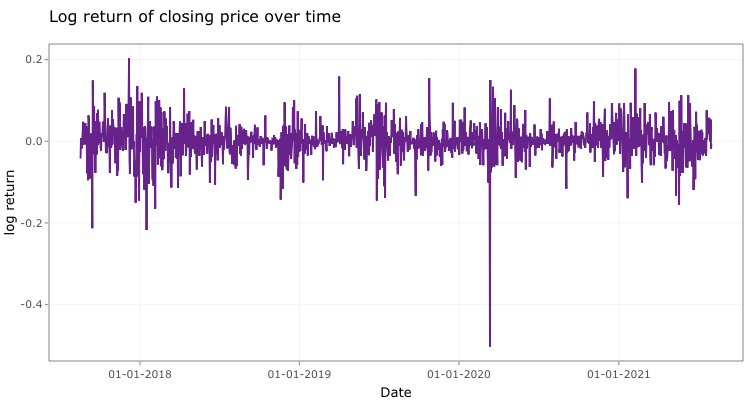
\includegraphics[width=\linewidth]{Extremal Modelling/logreturn_17_21.png}
    \caption{The daily log return of Bitcoin process from August 2017 to August 2021. Notice the very large drop in March of 2020.}
    \label{fig:logreturn_17_21}
\end{figure}

In light of this, it is not unnatural to ask the corresponding statistical question in the context of extremes. In Figure \ref{fig:hist_logreturn_17_21}, we can see that the distribution of log returns for our data set admits very heavy tails. Admittedly, one is aware of the very large anomaly which greatly negatively skews the data in a noticeable fashion. However, in spite of this, using a common statistical rule for eliminating outliers based upon the quartiles of a distribution, we find, as in Figure \ref{fig:distplots_sans_outliers}, the data still exhibits this skewed behaviour. This sparks interest in using extreme value theory to aid our understanding of it.\\

Let $(X_i)_{i=1}^n$ be a random sample from some distribution $F$, and $M_n = \max(X_1, \ldots, X_n)$ be the $n$th order statistic. If there exist sequences $(a_n) \subset \mathbb{R}^+$ and $(b_n) \subset \mathbb{R}$ such that $(M_n - b_n)/a_n \overset{D}{\to} G$, for some distribution $G$, then $G$ must be of extremal value type, that is, \[
G(x; \eta, \tau, \xi) = \begin{cases}
\exp\left[-\left\{1+\xi(x-\eta)/\tau\right\}_+\right], & \xi \ne 0\\
\exp\left[-\exp\left\{-(x-\eta)/\tau\right\}\right], & \xi = 0
\end{cases}
\]
where $\eta, \tau$ and $\xi$ are location, shape and scale parameters respectively. \begin{remark}
Extreme value theory does not apply singly to maxima, if $M_n' = \min(X_1, \ldots, X_n)$, then we have that $M_n' = -\max(-X_1, \ldots, -X_n)$ and so the corresponding limiting distribution function is $1-G(-x)$. 
\end{remark}

Studying maxima in this way is known as the \textbf{block maxima approach}, since one groups data and considers fitting the distribution to the maxima across all groups, for example: annual global extreme temperatures. There is another approach, called \textbf{peaks over thresholds}, which studies the exceedance of a random sample beyond a predefined threshold. This will be discussed later.


The goal now, therefore, is to fit this model to our data, i.e. by finding the unknown parameters. To this end, we use the $\code{R}$ package $\code{evd}$ which gives useful functions for extremal modelling and makes plotting diagnostics straightforward. The function $\code{fgev}$ fits the block maxima (or minima when appropriately transformed) to the model through maximum likelihood estimation. Assuming certain regularity conditions, we can derive estimates and corresponding uncertainties from our method.  
\begin{figure}
    \centering
    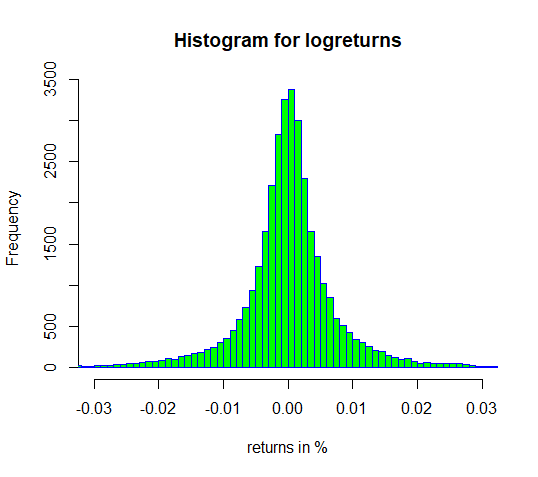
\includegraphics[width=\linewidth, height=3.5in]{TestPlots/Histogram log-returns2.png}
    \caption{Distribution of log returns using data from August 2017 to August 2021. The distribution shows some quite heavy tails.}
    \label{fig:hist_logreturn_17_21}
\end{figure}

\begin{figure}
    \centering
    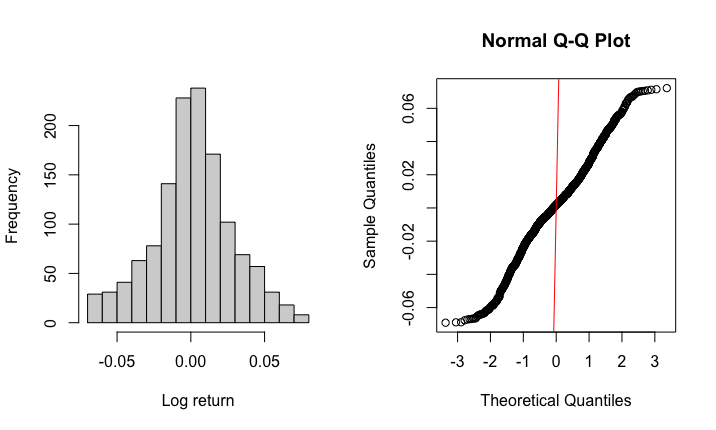
\includegraphics[width=\linewidth]{Extremal Modelling/distplots_sans_outliers.png}
    \caption{Distribution of log returns having eliminated outliers and a QQ plot of the data against a standard normal random variable. Clearly the data is still heavily tailed.}
    \label{fig:distplots_sans_outliers}
\end{figure}










\end{spacing}
\end{document}
